\section{Annexes}
\label{appendix}
\appendix

\newpage
\section*{Définitions des événements d'une politique}
\begin{figure}[h!t]
    \centering
    \begin{tabular}{c}
        \begin{lstlisting}[language=Phaistos, linewidth=13cm]
EVENTS {
    On INIT() do: {
        init(POLICY.fifo_list[READ]); 
        init(POLICY.fifo_list[WRITE]);
        ...
        POLICY.fifo_expire[READ]=read_expire;
        POLICY.fifo_expire[WRITE]=write_expire; 
        POLICY.fifo_batch = fifo_batch;
        POLICY.writes_starved = writes_starved;
        POLICY.starved = 0;
        POLICY.batching = 0;
    }
    On DISPATCH(request rq) do: {
        bool reads; 
        bool writes;
        reads = !is_empty(POLICY.fifo_list[READ]);
        writes = !is_empty(POLICY.fifo_list[WRITE]);
        if(rq && POLICY.batching < POLICY.fifo_batch) {
            POLICY.batching++;
            return rq;
        }
        if(reads) {
            if (deadline_fifo_request(WRITE) &&
            POLICY.starved++ >= POLICY.writes_starved) {
                return dispatch_writes();
            }
            return dispatch_reads();
        }
        if(writes) {
            return dispatch_writes();
        }
        return rq; 
    }
    ...
}
        \end{lstlisting}
    \end{tabular}
    \caption{Exemple d'une définition des événements \texttt{INIT} et \texttt{DISPATCH} écrits dans le langage du DSL pour la politique Deadline.}
    \label{fig:event-code}
\end{figure}

\newpage
\section*{Arborescence du projet}
\begin{figure}[h!t] \centering
    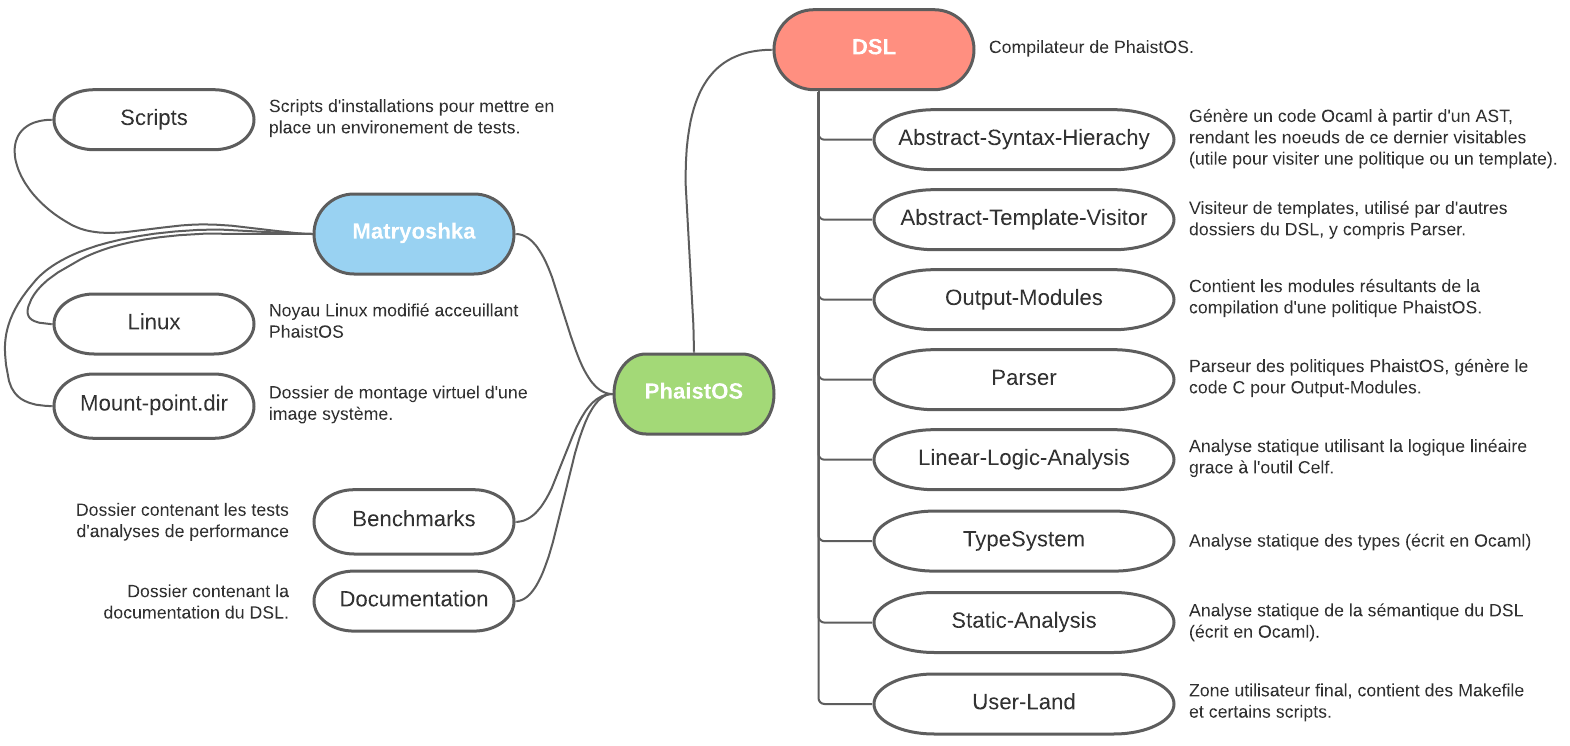
\includegraphics[width=\textwidth]{images/arch}
    \caption{Architecture du projet PhaistOS.}
    \label{fig:arch}
\end{figure}

\newpage
\section*{Les politiques d'ordonnancement de Linux}
\begin{table}[h!t]
    \begin{tabularx}{\textwidth} { 
        | >{\hsize=0.22\hsize\linewidth=\hsize\raggedright\arraybackslash}X 
        | >{\hsize=0.26\hsize\linewidth=\hsize\raggedright\arraybackslash}X 
        | >{\hsize=1.51\hsize\linewidth=\hsize\arraybackslash}X | }
        \hline
        \textbf{Nom} & \textbf{Catégorie de file d'attente} & \textbf
        {Description} \\
        \hline
        \hline
        Deadline & Simple & Conçu pour régler les problèmes de famine aperçu 
        dans d'autres ordonnanceurs à l'époque. Son algorithme utilise 3 files, 
        à savoir une file dite ``triée'' (par priorité), une file de lecture et 
        une file d'écriture. Les requêtes de la file triée sont prioritaires et 
        si une des requêtes des deux autres files expire, elle devient 
        prioritaire. Les lectures ont un délai d'expiration de 0.5s par défaut 
        tandis que les écritures sont moins privilégiées avec 5s d'expiration. 
        \\
        \hline
        CFQ & Simple & Conçu pour se rapprocher des processus. Possède des 
        files distinctes par processus et se base sur la valeur ``ionice'' pour 
        les priorités. Chaque file se voit attribuer un temps d'équité, pouvant 
        provoquer ainsi des situation de ``vide'' si le temps attribué n'est 
        pas utilisé. \\
        \hline
        Noop & Simple & Aucun tri n'est effectué avec cet algorithme 
        d'ordonnancement, seulement des fusions de requêtes aux adresses 
        voisines. Il peut être efficace dans de rare cas, mais cela inclu les 
        contrôleurs de stockage avancés, qui trient eux-même leur requêtes \\
        \hline
        BFQ (Budget Fair Queuing) & Multiple & Conçu pour fournir une bonne 
        réponse interactive, en particulier pour les périphériques d'E/S lents. 
        Il n'est cependant pas idéal pour les périphériques dotés de 
        processeurs lents car chaque opération entraine une surchage de travail 
        assez élévée. La notion d'équité ici repose sur la taille des données 
        demandées plutôt que sur le temps. \\
        \hline
        Kyber & Multiple & Créé pour les périphériques multi-files rapides 
        comme les disques SSD ou les cartes \texttt{M.2} par exemple. Il reste 
        relativement simple et distribue les requêtes dans deux files : celle 
        des lectures et celle des écritures. Grâce à sa limitation du nombre de 
        requêtes pouvant être traitées à la fois, Kyber offre un temps de 
        service rapide pour les requêtes à haute priorités \cite{Kyber}. Il 
        sera souvent retrouvé comme ordonnanceur pour des serveurs, cependant 
        pour des machines avec un processeur plus lent, on retrouvera BFQ ou 
        MQ-Deadline. \\
        \hline
        None & Multiple & C'est tout simplement l'ordonnanceur qui n'en est pas 
        un. Aucune réorganisation des requêtes n'est effectuée, procurant ainsi 
        une surcharge minimale. Il peut être utile pour certains appareils très 
        rapides utilisant les technologies NVMe, comme les disques SSD. \\
        \hline
        MQ-Deadline & Multiple & C'est la version multi-files de l'algorithme 
        ``Deadline'', polyvalent, il reste le plus souvent utilisé dû à sa 
        faible surcharge CPU.\\
        \hline
    \end{tabularx}
    \caption{Les différentes politiques d'ordonnancement de Linux}
    \label{tab:politics}
\end{table}
  